\section{Fabrication and deployment}
 \begin{figure}[h!]
 	\includegraphics[height=10.5cm]{figure1}
 	\caption{\small Geometry and naming convention of a dipole qubit. a) Scanning electron image of the dipole structure with labeled assymetric flux bias (carried by dimensionless $ \eta $) $ \Phi $, $ \eta\Phi $ applied to its superconducting loops. The dipoles are of macroscopic size, $ > 20\,\mu $m and coupled capacitively to a $ Z_0 = \iunit{50}{$ \Omega $} $ microwave line (inset); b) The state of the 5 JJs are unqiuely defined by thee phases, $ \varphi_{1}, \varphi_{2}, \varphi_{3}$ and $ \varphi_0 = 0$ which is grounded. The central junction has a boosted $ \alpha E_J $, $ \alpha C $ energy and capacitance relative to the outside JJs.}
 	%\caption{\small{Scanning electron microscope image of the dipole qubits capacitively coupled to the tranmisssion line. A common flux $ \Phi $ is applied to each loop with an external magnetic field. This magnetic field effects the phases induced across the junction$ \phi_i$ .} Phases will arange is such a way, so that potential energy is minimised}
 	\label{fig:setup}
 \end{figure}
 
 %%Describe fabrication
 The structure is made by coating an undoped silicon with gold film, and patterning out a coplanar transmission line, with impedance $ Z \approxeq 50\,\Omega $, leading to an opening in the center of the chip. Dipole qubits loops are deposited in this region using shadow evaporation of aluminium, along with the T-shaped capacitors through which driving microwaves are coupled. Results were obtained for one of the dipoel qubits, which has $ \red{E_J\sim \iunit{91}{GHz}} $ and \red{$ E_C \sim \iunit{23}{GHz} $} ($ \text{Area}_\text{JJ} \sim 200\times 400\,\text{nm}^2$). The tranistions between the lowest levels $ \omega_{21} $ and $ \omega_{32} $ fell within the accesible 1\,-\,40\,GHz frequency range of our low-noise microwave setup. The experiment is performed in a 14\,mK environment to supress thermal activation.


 %% Desribe what was measured
 The qubit is coupled to the transmission line through the capacitor, $ C $. A weak probing frequency, $ f $, is swept, while an external magnetic field, linking fluxes $ \Phi $ and $ \eta\Phi $ through the left and right loops of the dipole, controlling the energy levels. The spectrum is not periodic in $ \Phi $, due to the assymetry $ \eta $ between the loops, see Fig.~\ref{fig:experiment}. The spectrum is mapped out by selecting the strongest resonanances in this flux-frequency plane. The measurement done using two-tone spectroscopy: signal from the VNA generator at $ \omega_{21} $ creates population inversion \iket{1}$ \,\rightarrow\,$\iket{2} while the second high frequency generator applies $ \omega_{32} $. Whenever the \iket{2}$ \,\rightarrow\,$\iket{3} transition is hit, we detect a VNA transmission amplitude change, allowing us to reach levels beyond the range of out 20\,GHz instruments. 
 
 %%%%%
 % image of experimental result
 %%%%%
 \begin{figure}[h!]
 	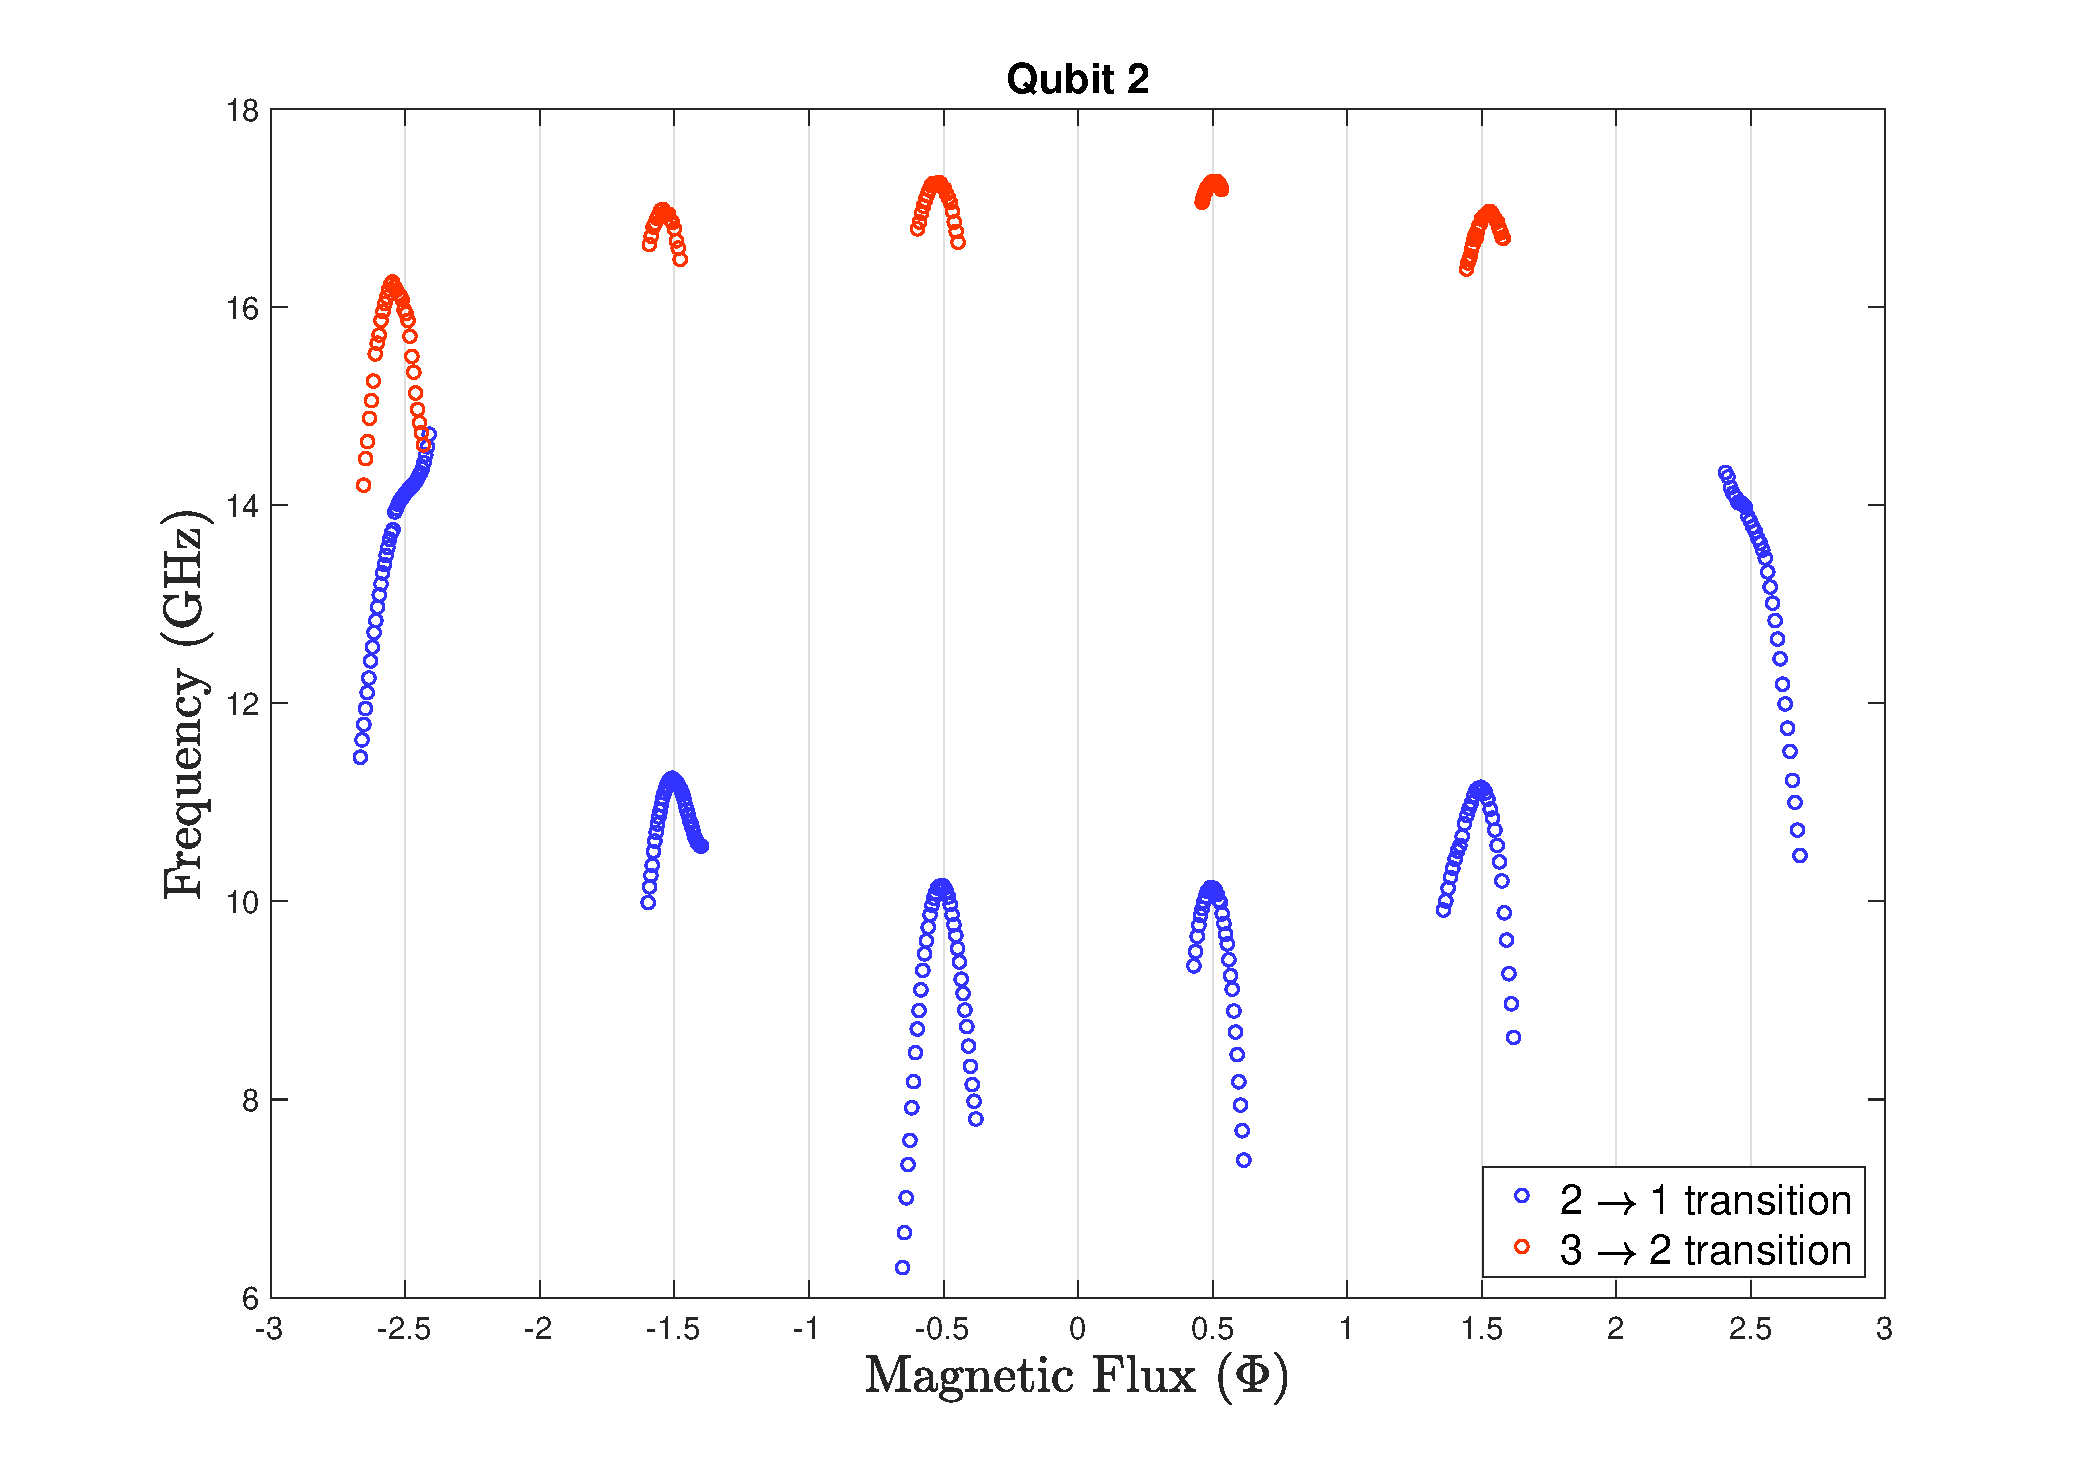
\includegraphics[height=5.5cm]{figure2_qubit2}	
 	\caption{Transition energies of the dipole qubit. The VNA generator weakly drives the $ \iket{1}\,\ra\,\iket{2} $ transition, while the generator sends if a strong $ \iket{2}\,\ra\,\iket{3} $ tone. Assymetry in the flux penetrating the left and right loops results in the creeping of the energy levels with a period $ \Phi_0 $ and offset of the $ \iket{2}\,\rightarrow\,\iket{3} $ transition. The rise of the outermost $ \omega_{21} $ transition is caused by the \red{interaction with the $ \omega_{32} $ transition}. \label{fig:experiment}
 	}%The magnetic field was swept, and the maxima were taken down using a point by point readout scheme. Two-tone spectroscopy was used to obtain the $ \omega_{32} $ data, in which a VNA drove the $ \omega_{21} $ transition, and a generator drove the $ \omega_{32} $ transition. A $ 2\lra 3 $ transition would manifest itself in a change of the VNA transmission.}
 \end{figure}